\chapter{Background}
\label{chap:background}

XXX We need to decide, y'know, what goes into the background section.

What did we say in the outline?

\begin{itemize}
\item history of CL-WSD
\item related work
\item Guarani language
\item maybe Quechua and Amharic languages too!
\end{itemize}

\section{Word-Sense Disambiguation}

% XXX
Word types often -- or perhaps always, to take a philosophical view of 
communication and semiosis -- have many possible meanings. Given a string of
characters or an utterance, there are many possible meanings that one
could assign to that word token. In the simplest case, one could be faced with
a homophone or homograph and need to distinguish between different lexemes that
could be intended. There could be technical or jargon senses that conflict with
colloquial uses of a word; consider the many different meanings of ``kernel",
``type" and ``kind" in computer science and mathematics. In the most difficult
case, the usages can be hyperbolic, metaphorical, sarcastic, or oblique
references. Understanding these usages will require understanding the broader
discourse context and the goals of the speaker, which is outside the scope of
this work.

More simply, when faced with a token in a piece of text, we want to be able to
label which \emph{word sense} from a \emph{sense inventory} is meant. The sense
inventory might come from a pre-set ontology built by lexicographers, such as a
dictionary or a WordNet.
%XXX

For a broad overview of the history of word sense disambiguation, please see
Navigli \emph{et al.}'s book on the topic. \cite{wsdbook}


It has long been held that word sense disambiguation is a central problem in
other NLP applications, including machine translation. As early as 1960,
Yehoshua Bar-Hillel considered machine translation for the general case to be
impossible, due to the insurmountable task of writing WSD routines for all
source-language words. \cite{barhillel1960}

\begin{quote}
During the past year I have repeatedly tried to point out the illusory
character of the FAHQT ideal even in respect to the mechanical determination of
the syntactical structure of a given source-language sentence... Here I shall
show that there exist extremely simple sentences in English -- and the same
holds, I am sure, for any other natural language -- which within certain
linguistic contexts, would be uniquely (up to plain synonymy) and unambiguously
translated into any other language by anyone with a sufficient knowledge of the
two languages involved, though I know of no program that would enable a machine
to come up with this unique rendering unless by a completely arbitrary and
\emph{ad hoc} procedure whose futility would show itself in the next example.

A sentence of this kind is the following: \emph{The box was in the pen.}
\end{quote}

\section{Cross-lingual word sense disambiguation}
\label{sec:clwsd}

Cross-lingual word sense disambiguation (CL-WSD) is the task of labeling words
or phrases in some input text with their contextually-appropriate translations
into some target language.
It is a variant of the more general WSD task, with the sense inventory for each
word defined as its possible translations.
This setting for WSD has immediate applications in both machine translation and
cross-language information retrieval, since many words have multiple possible
translations.

WSD in translation has a long history; practical work in integrating
WSD with statistical machine translation dates back to early SMT work at IBM
\cite{Brown91word-sensedisambiguation}, but the problem itself was described in
Warren Weaver's prescient 1949 memorandum \cite{weavermemo}, which describes an
essentially modern conception of word sense disambiguation.

In the early history of machine translation, researchers were very concerned
with WSD; to some, it seemed an insurmountable problem. Bar-Hillel 
discussed the difficulty of writing a program to translate sentences with
simple ambiguities like \emph{The box was in the pen.} \cite{barhillel1960}:

\begin{quote}
... I know of no program that would enable a machine to come up with this
unique rendering unless by a completely arbitrary and ad hoc procedure whose
futility would show itself ...
\end{quote}

To produce a correct rendering of this sentence in Spanish, for example, the
translation system must decide between translating ``pen" as \emph{corral} (an
enclosure, like for an animal) or as \emph{pluma} (the instrument for writing).
As of this writing, for this particular example, Google Translate picks the
less-sensible ``in the writing implement" translation (see Figure
\ref{fig:box-in-pen}).
One wonders how this could come about -- we would hope that the n-gram language
model for Spanish would prefer sentences about things in enclosures to things
in writing implements.
But the word \emph{en} can be a translation of either the English ``in" or
``on", and \emph{pluma} can also mean ``feather".
The situation is fairly complex.


\begin{figure}
  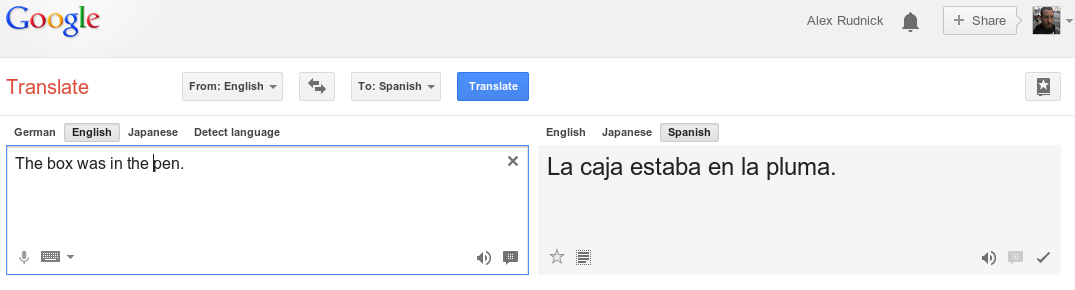
\includegraphics[width=12cm]{box-in-pen.png}
  \caption{Google Translate, September 17, 2013; interestingly, adding or
  removing the final period in the English sentence causes a switch between the
  ``pluma" and ``corral" renderings.}
  \label{fig:box-in-pen}
\end{figure}

In general, there is a many-to-many relationship between words across language
boundaries.
This happens for a number of reasons: figurative or metaphorical uses may not
translate directly,
obligatory information in one language may be left unspecified in another,
or the criteria for selecting a word may simply differ.
To give some familiar examples, a ``leg" of a trip in English is typically
translated as \emph{etape} in French, which is unrelated to limbs used for
walking;
translating ``brother" to Japanese requires specifying whether the brother is
older (\emph{ani}) or younger (\emph{ot\=oto});
a soap bubble or a ceramic plate can be destroyed with the same word in
Chinese, whereas English speakers typically distinguish between the verbs
``pop" and ``break" \cite{majid2007semantic}.

Despite these difficulties, most statistical MT systems do not use an explicit
WSD module \cite{wsdchap3}; the language model and phrase tables of these
systems mitigate lexical ambiguities by encouraging words used collocationally
to appear together in the output. Entire phrases\footnote{Not necessarily
``phrases" in a syntactic sense, but subsequences of sentences} such as verbs
with their common objects may be learned and stored in the phrase table, and
the language model will encourage common collocations as well.

To take a look at some apparently easier examples, let us also consider the
following usages of \emph{letter}, from the test set of a recent SemEval shared
task \cite{task10}, and how to translate them into Spanish.

\enumsentence{
But a quick look at today's \emph{letters} to the editor in the Times suggest
that here at least is one department of the paper that could use a little more
fact-checking. }
\label{sent:carta}
\enumsentence{
All over the ice were little Cohens, little Levys, their names sewed in block
\emph{letters} on the backs of their jerseys. }
\label{sent:letra}

We would want (\ref{sent:carta}) to be translated with the word \emph{carta},
and (\ref{sent:letra}) to be translated with \emph{letra} or something similar.
Google Translate (as of this writing) handles both of these sentences well,
rendering the first with ``cartas" and the second with an even better choice,
translating the phrase ``block letters" as \emph{mayúsculas}.
However longer-distance relationships, search errors, or simple statistical
accidents can still cause strange translations in practice.

Despite the great success of SMT systems without any explicit models for WSD,
there has been recent interest in CL-WSD and its application to translation
systems, sparking shared tasks at recent SemEval workshops
\cite{lefever-hoste:2010:SemEval,task10} and a number of other projects
described in some detail in \S\ref{sec:relatedwork}).

In this dissertation, we will describe in detail some new approaches for CL-WSD
and how to integrate them into a practical machine translation system.
We will develop and extend at least two broad approaches for CL-WSD: the use of
multilingual evidence where available, and CL-WSD as a sequence labeling
problem.
Both of these techniques have been prototyped and presented at workshops, but
they will be refined significantly and packaged into more general tools for use
in MT.  

\begin{figure}
  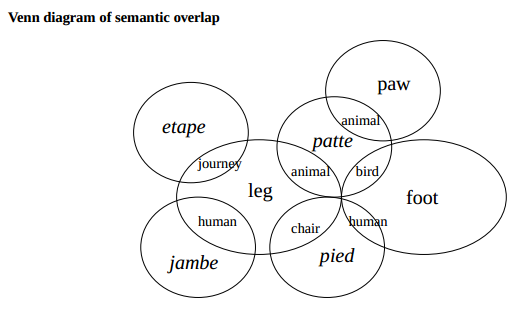
\includegraphics[width=12cm]{hutchins-leg-etc.png}
  \caption{Overlap of words related to ``leg"; relationships between English
  and French words. Figure 21.2 from \protect\cite{slp1}; example originally
  from \protect\cite[Chapter 6]{hutchins1992introduction}.}
  \label{fig:leg}
\end{figure}









\section{Hybrid MT}

In recent years, we have seen renewed interest in machine translation systems
that take into account syntactic structure, linguistic knowledge, and semantic
representations.
Hopefully, these will provide better translation for language pairs with
significant reordering or syntactic divergences, and where one or both of the
languages has rich morphology.
The boundaries between rule-based and statistical MT systems are becoming
increasingly blurred, and hybrid systems are being developed in both
directions, with RBMT systems incorporating components based on machine
learning, as well as SMT systems making use of linguistic knowledge for
morphology and syntax.

Additionally, for most of the world's language pairs, there is simply no large
bitext corpus available, so training a purely statistical machine translation
system is infeasible.
Thus, while SMT approaches have had great success, and drastically changed the
machine translation landscape since the 1990s, RBMT approaches are still
relevant for many language pairs.

We would like for RBMT or hybrid systems, once developed, to be able to make
use of any bitext on hand.  Like SMT systems, they should be able to produce
better translations as larger corpora become available, without additional code
changes.
In this dissertation work, we will develop a software package called
chipa, which will do just that: %% XXX: better wording?
it will integrate with a variety of machine translation systems to help them
use any available bitext to make better word choices.







\section{History of CL-WSD}


ParaSense, the CL-WSD system developed by Els Lefever
\cite{lefever-hoste-decock:2011:ACL-HLT2011}, takes into account evidence from
several different parallel corpora.
For predicting the translation of a source word into
any particular target language, ParaSense creates
bag-of-words features from the translations of the input sentence into every
other language that it knows about. As of this writing, ParaSense handles
translation from English into French, Spanish, Italian, Dutch and German.
Given corpora that are parallel over many languages, such as Europarl, this is
straightforward at
training time. However, at testing time it requires a complete MT system for
each of the four other languages, which seems computationally prohibitive. In
the past, ParaSense has simply called out to the Google Translate API to
generate the bag-of-words features required for test sentences. This seems
unwieldy, and thus in our work, we learn from several parallel corpora but
require neither a locally running MT system nor access to an online translation
API.

To our knowledge, there has not been other work on framing CL-WSD for all words
in an input sentence as a sequence labeling problem. However, in monolingual
WSD, Molina \textit{et al.} \cite{DBLP:conf/iberamia/MolinaPS02} have made
use of HMMs for WSD. 


\section{CL-WSD for Lexical Selection}
While most SMT systems do not make use of an explicit WSD module, recently
there has been work on adding WSD classifiers in to statistical MT systems.
Particularly, Carpuat and Wu have shown how to use CL-WSD, or more broadly,
cross-lingual phrase sense disambiguation, to improve modern phrase-based SMT
systems
\cite{carpuatpsd,carpuat-wu:2007:EMNLP-CoNLL2007,carpuat2008evaluation}. In
Carpuat's work, classifiers are used to label multi-word expressions (phrases,
in the phrase-based SMT sense) with target language phrases. She demonstrates
how this is more appropriate in an an SMT setting than simply labeling
individual words with WordNet synsets, as had previously been attempted, and
showed significant improvements on a Chinese-English translation task.

There has also been work on using discriminative MaxEnt models to adapt
the ``forward" translation model of an SMT system, using richer
source-language context features \cite{vzabokrtsky-popel-marevcek:2010:WMT}.
Somewhat interestingly, while it has the same effect, this work does not
describe itself in terms of word sense disambiguation.

%% text from the HyTra paper
Although they did not present a complete MT system, there has also been work
on using WSD techniques for translation into lower-resourced languages, such as
the English-Slovene language pair, as in
\cite{vintar-fivser-vrvsvcaj:2012:ESIRMT-HyTra2012}. 

%%The Apertium team has a particular practical interest in improving lexical
%%selection in RBMT; they recently have been developing
%%a new system, described in \cite{tyers-fst}, that learns finite-state
%%transducers for lexical selection from the available parallel corpora. It is
%%intended to be both very fast, for use in practical translation systems, and
%%to produce lexical selection rules that are understandable and modifiable by
%%humans.

Francis Tyers, in his dissertation work \cite{tyers-dissertation},
provides an overview of lexical selection systems and describes methods for
learning lexical selection rules based on available parallel corpora.
These rules make reference to the lexical items and parts of speech surrounding
the word to be translated. Once learned, these rules are intended to be
understandable and modifiable by human language experts. For practical use in
the Apertium machine translation system, they are compiled to finite-state
transducers.


\section{Online Language Tools for Guarani}
There are currently very few online language tools for Guarani; some of the
best available ones are iGuarani \footnote{\url{http://iguarani.com/}}, a
searchable online dictionary and gisting translation system developed by young
Paraguayan programmer Diego Alejandro Gavilán.

There is also a small searchable online dictionary developed by Wolf Lustig
\footnote{\url{http://www.uni-mainz.de/cgi-bin/guarani2/dictionary.pl}},
which has versions in Spanish, German, and English. He has graciously made this
dictionary available for our use, and this will provide a starting point for
our Spanish-Guarani translation system.

The Guarani activist and education community has a presence on the Web,
although a startlingly large fraction of this presence is a single author,
Dr. David Galeano Olivera, the president of the \emph{Ateneo de Lengua y
Cultura Guaraní}. He has collected a number of resources both about and in the
Guarani language
\footnote{\url{http://cafehistoria.ning.com/profiles/blogs/la-lengua-guarani-o-avanee-en}},
some in Spanish and some in Guarani, and will likely continue to do so.





Here classifiers are trained with the scikit-learn machine learning package
\cite{scikit-learn}, using logistic regression (also known as ``maximum
entropy") with the default settings and the regularization constant set to
$C=0.1$. We also use various utility functions from NLTK \cite{nltkbook}. 

For this work, we use familiar features for text classification: the
surrounding lemmas for the current token (three on either side) and the
bag-of-words features for the entire current sentence. We additionally include,
optionally, the Brown cluster labels (see below for an explanation),
both for the immediate surrounding context and the entire sentence.
We suspect that more feature engineering, particularly making use of syntactic
information and surface word forms, will be helpful in the future.

\begin{figure}[t!]
  \begin{itemize}
    \item lemmas from surrounding context (three tokens on either side)
    \item bag of lemmas from the entire sentence
    \item Brown cluster labels from surrounding context
    \item bag of Brown cluster labels from the entire sentence
  \end{itemize}
\caption{Features used in classification}
\label{fig:features}
\end{figure}

\section{Related Work}

\subsection{early SMT with WSD}
%% Brown et al
Framing the resolution of lexical ambiguities in machine translation
as an explicit classification
task has a long history, dating back at least to early SMT work at IBM
\cite{Brown91word-sensedisambiguation}.

An early paper by IBM researchers \cite{Brown91word-sensedisambiguation},
outlines the CLWSD task in a strikingly similar way, as a WSD task where the
possible senses of a word are extracted from statistical alignments learned
over a bitext corpus. Brown \textit{et al.} report significant translation
quality improvements through the use of their WSD system, over a small
hand-evaluated set of test sentences.


\subsection{PB-SMT with phrase sense disambiguation}
%% Carpuat and Wu
More recently, Carpuat and Wu have
shown how to use classifiers to improve modern phrase-based SMT systems
\cite{carpuatpsd}.

Recent years have seen a resurgence of interest in the integration of
word-sense disambiguation techniques into machine translation.  We suspect that
WSD will be especially useful for translating into under-resourced and
morphologically rich languages, for which good language models are likely to be
sparse. Before the work of 
Carpuat and Wu~\cite{improvingsmtwsd}, it was apparently unclear whether
WSD was necessary or helpful for a state-of-the-art statistical MT system;
lexical choice among possible translations for a given word can often be
handled by the language model for the target language, simply due to
collocations of appropriate words in the training data.


\subsection{CL-WSD at SemEval}
CL-WSD has received enough attention to warrant shared tasks at recent SemEval
workshops; the most recent running of the task is described by Lefever and
Hoste \cite{task10}.
In this task, participants are asked to translate twenty different polysemous
English nouns into five different European languages, in a variety of contexts.


\subsection{multilingual evidence for CL-WSD}
%% ParaSense
Lefever \emph{et al.}, in work on the ParaSense system
\cite{lefever-hoste-decock:2011:ACL-HLT2011}, produced top results for
this task with classifiers trained on local contextual features, with the 
addition of a bag-of-words model of the translation of the complete source
sentence into other (neither the source nor the target) languages. At training
time, the foreign bag-of-words features for a sentence are extracted from
available parallel corpora, but at testing time, they must be
estimated with a third-party MT system, as they are not known a priori.
This work has not yet, to our knowledge, been integrated into an MT system
on its own.

Lefever \textit{et al.} recently described a novel approach to WSD, making use
of evidence from several languages at once to disambiguate English-language
source sentences. This is done by building artificial parallel corpora in
several languages, on demand, with the Google Translate API. They outperform
the previous state-of-the art systems on the SemEval 2010 shared task 13
\cite{lefever-hoste-decock:2011:ACL-HLT2011}.

In our earlier work, we prototyped a system that addresses some of the issues
with ParaSense, requiring more modest software infrastructure for feature
extraction while still allowing CL-WSD systems to make use of several mutually
parallel bitexts that share a source language
\cite{rudnick-liu-gasser:2013:SemEval-2013}.

\subsection{WSD for lower-resourced languages}
However, there has been work recently on using WSD techniques for translation
into lower-resourced languages, such as the English-Slovene language pair, as
in \cite{vintar-fivser-vrvsvcaj:2012:ESIRMT-HyTra2012}. 

Dinu and Kübler~\cite{Dinu07} have addressed the problem of monolingual WSD for
a lower-resourced language, particularly Romanian. In their work, they describe
an instance-based approach in which a relatively small number of features is
used quite effectively. In other work on lower-resourced languages,
Sarrafzdadeh \textit{et al.} have investigated a version of the Lesk algorithm
for Farsi.

%% XXX
One sort of interesting point here is that we are not doing WSD on a
low-resourced language. This is ultimately WSD on Spanish with a sense
inventory that we automatically discover from cross-lingual evidence.

\subsection{lexical selection in low-resource settings}
Francis Tyers, in his dissertation work \cite{tyers-dissertation},
provides an overview of lexical selection systems and describes methods for
learning lexical selection rules based on available parallel corpora. These
rules make reference to the lexical items and parts of speech surrounding the
word to be translated. Once learned, these rules are intended to be
understandable and modifiable by human language experts. For practical use in
the Apertium machine translation system, they are compiled to finite-state
transducers.

The Apertium team has a particular practical interest in improving lexical
selection in RBMT; they recently have been developing
a new system, described in \cite{tyers-fst}, that learns finite-state
transducers for lexical selection from the available parallel corpora. It is
intended to be both very fast, for use in practical translation systems, and
to produce lexical selection rules that are understandable and modifiable by
humans.

%% SQUOIA extensions: relevant to Hybrid MT
Rios and G\"{o}hring \cite{riosgonzales-gohring:2013:HyTra} describe
earlier work on extending the SQUOIA MT system with machine learning modules.
They used classifiers to predict the target forms of verbs in cases where the
system's hand-crafted rules cannot make a decision based on the current
context.

\subsection{Sequence models for word-sense disambiguation}
To our knowledge, there has not been work specifically on sequence labeling
applied to lexical selection for RBMT systems.

Outside of the CL-WSD setting, there has been work on framing all-words WSD as
a sequence labeling problem. Particularly, Molina \textit{et al.}
\cite{DBLP:conf/iberamia/MolinaPS02} have made use of HMMs for all-words
WSD in a monolingual setting.

We have also done some previous work on CL-WSD for translating into indigenous
American languages; an earlier version of Chipa, for Spanish-Guarani, made use
of sequence models to jointly predict all of the translations for a sentence at
once \cite{rudnick-gasser:2013:HyTra}.



\subsection{Translation into Morphologically Rich Languages}
Chris Dyer's recent paper at EMNLP
\cite{chahuneau:2013:emnlp}

Talk about prediction for morphology.
\cite{toutanova-suzuki-ruopp:2008:ACLMain}

Also factored models...
\cite{yeniterzi-oflazer:2010:ACL}


\chapter{Related Work}
\label{sec:relatedwork}

\section{CL-WSD \emph{in vitro}}
ParaSense, the CL-WSD system developed by Els Lefever
\cite{lefever-hoste-decock:2011:ACL-HLT2011}, takes into account evidence from
several different parallel corpora.
For predicting the translation of a source word into
any particular target language, ParaSense creates
bag-of-words features from the translations of the input sentence into every
other language that it knows about. As of this writing, ParaSense handles
translation from English into French, Spanish, Italian, Dutch and German.
Given corpora that are parallel over many languages, such as Europarl, this is
straightforward at
training time. However, at testing time it requires a complete MT system for
each of the four other languages, which seems computationally prohibitive. In
the past, ParaSense has simply called out to the Google Translate API to
generate the bag-of-words features required for test sentences. This seems
unwieldy, and thus in our work, we learn from several parallel corpora but
require neither a locally running MT system nor access to an online translation
API.

To our knowledge, there has not been other work on framing CL-WSD for all words
in an input sentence as a sequence labeling problem. However, in monolingual
WSD, Molina \textit{et al.} \cite{DBLP:conf/iberamia/MolinaPS02} have made
use of HMMs for WSD. 

%%\subsection{Translation into Morphologically Rich Languages}
%%Chris Dyer's recent paper at EMNLP
%%\cite{chahuneau:2013:emnlp}
%%Talk about prediction for morphology.
%%\cite{toutanova-suzuki-ruopp:2008:ACLMain}
%%Also factored models...
%%\cite{yeniterzi-oflazer:2010:ACL}

\section{CL-WSD for Lexical Selection}
While most SMT systems do not make use of an explicit WSD module, recently
there has been work on adding WSD classifiers in to statistical MT systems.
Particularly, Carpuat and Wu have shown how to use CL-WSD, or more broadly,
cross-lingual phrase sense disambiguation, to improve modern phrase-based SMT
systems
\cite{carpuatpsd,carpuat-wu:2007:EMNLP-CoNLL2007,carpuat2008evaluation}. In
Carpuat's work, classifiers are used to label multi-word expressions (phrases,
in the phrase-based SMT sense) with target language phrases. She demonstrates
how this is more appropriate in an an SMT setting than simply labeling
individual words with WordNet synsets, as had previously been attempted, and
showed significant improvements on a Chinese-English translation task.

There has also been work on using discriminative MaxEnt models to adapt
the ``forward" translation model of an SMT system, using richer
source-language context features \cite{vzabokrtsky-popel-marevcek:2010:WMT}.
Somewhat interestingly, while it has the same effect, this work does not
describe itself in terms of word sense disambiguation.

%% text from the HyTra paper
Although they did not present a complete MT system, there has also been work
on using WSD techniques for translation into lower-resourced languages, such as
the English-Slovene language pair, as in
\cite{vintar-fivser-vrvsvcaj:2012:ESIRMT-HyTra2012}. 

%%The Apertium team has a particular practical interest in improving lexical
%%selection in RBMT; they recently have been developing
%%a new system, described in \cite{tyers-fst}, that learns finite-state
%%transducers for lexical selection from the available parallel corpora. It is
%%intended to be both very fast, for use in practical translation systems, and
%%to produce lexical selection rules that are understandable and modifiable by
%%humans.

Francis Tyers, in his dissertation work \cite{tyers-dissertation},
provides an overview of lexical selection systems and describes methods for
learning lexical selection rules based on available parallel corpora.
These rules make reference to the lexical items and parts of speech surrounding
the word to be translated. Once learned, these rules are intended to be
understandable and modifiable by human language experts. For practical use in
the Apertium machine translation system, they are compiled to finite-state
transducers.

\section{Online Language Tools for Guarani}
There are currently very few online language tools for Guarani; some of the
best available ones are iGuarani \footnote{\url{http://iguarani.com/}}, a
searchable online dictionary and gisting translation system developed by young
Paraguayan programmer Diego Alejandro Gavilán.

There is also a small searchable online dictionary developed by Wolf Lustig
\footnote{\url{http://www.uni-mainz.de/cgi-bin/guarani2/dictionary.pl}},
which has versions in Spanish, German, and English. He has graciously made this
dictionary available for our use, and this will provide a starting point for
our Spanish-Guarani translation system.

The Guarani activist and education community has a presence on the Web,
although a startlingly large fraction of this presence is a single author,
Dr. David Galeano Olivera, the president of the \emph{Ateneo de Lengua y
Cultura Guaraní}. He has collected a number of resources both about and in the
Guarani language
\footnote{\url{http://cafehistoria.ning.com/profiles/blogs/la-lengua-guarani-o-avanee-en}},
some in Spanish and some in Guarani, and will likely continue to do so.


